\subsubsection{Minuta de reunião (19-Agosto-2015)}

\begin{tabbing}
  Local \= xxx \kill
  Local \> : LEAD \\
  Data  \> : 19 de Agosto de 2015 \\
  Hora  \> : 13:00
\end{tabbing}

%---------------------------------------------------------------------
\participantes{
  \gabriel,
  \julia,
  \estevão,
  \ramon.

}

\textbf{Aprovação da minuta}

\textbf{Update semanal do Projeto EMMA}
   							
					
\textbf{\gabriel.} 
	\begin{itemize}
		\item Escolher equipamento para calibração.
				\item Usou ROS e ROCK com LMS111 Laser scan, porém nenhum funcionou bem.
				\item Reunião Nikon Metrology: eles podem nos fornecer a solução completa
				para calibração, porém precisam de pelo menos 2.5 metros de distância
				dos alvos para fazerem a leitura.
				\item Reunião com FARO essa semana.
			\end{itemize}
		
		\item \textbf{Novas tarefas:}
			\begin{itemize} 
				\item Reunião com FARO.
				\item Implementar o driver do ROS no ROCK para fazer o Laser Scan LMS111
				funcionar bem.
			\end{itemize}

					
			
   \textbf{\estevão.} 
	\begin{itemize}
		\item \textbf{Tarefas concluídas:}
			\begin{itemize}    
				\item Desenhou o modelo da maquete, pediu cotações para as peças que
				queremos imprimir 3D. Apenas a pá sairia entre 5 e 7 mil reais, resultando
				em um valor muito alto. 
				\item Conversou com prossor da EBA sobre a possiblidades de fazer a maquete.
				\item Desenho dos braços sem os graus de liberdade apresentou problema co
				relação ao acesso dos cabos por cima quando o robô estiver na frente da pá.
				
			\end{itemize}
		
		\item \textbf{Novas tarefas:}
			\begin{itemize} 
			    \item Continuar estudo da solução da escotilha inferior com Renan.
			    \item Fazer estudo se teremos de conectar e desconetar os cabos toda vez
			    que tivermos de girar o rotor.
				\item Atualização do modelo maquete.
			    \item Solid works: Desnehar o lipe da pá.
			\end{itemize}
	\end{itemize}

	  \textbf{\Renan.} 
	\begin{itemize}
		\item \textbf{Tarefas concluídas:}
			\begin{itemize}    
				\item Fez um estudo da dos tolerancia no end effector. 
			\end{itemize}
		
		\item \textbf{Novas tarefas:}
			\begin{itemize} 
			    \item Formalizar no SOTA. 
			\end{itemize}
	\end{itemize}		
			
			
   \textbf{\Julia.} 
	\begin{itemize}
		\item \textbf{Tarefas concluídas:}
			\begin{itemize}    
				\item Proposta de Mestrado para PUC e UFRJ.
				\item Metodologia de Interface Gráfica do controle de missão do projeto.
			\end{itemize}
		
		\item \textbf{Novas tarefas:}
			\begin{itemize} 
			    \item Continuar trabalho de metodologia e apresenta-los para os
			    integrantes da equipe que estavam no congresso CITENEL.
			    \item Buscar Engenheiro de software para o projeto. (processo de
			    seleção a ser discutido).
			\end{itemize}
	\end{itemize}		



\textbf{Agenda para a próxima reunião:}
  \begin{itemize}
    \item Resultado de pesquisas individuais.
    \item Novas tarefas \& recomendações.
  \end{itemize}


\vspace{5mm}%
\parbox[t]{70mm}{
  Aprovado por: \\[5mm]
  \centering
  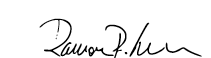
\includegraphics[width=65mm]{figs/logo/assinatura-ramon.png} \\[-4mm]
  \rule[2mm]{70mm}{0.1mm} \\
  \ramon \\[1mm]
  Coordenador do Projeto \\
}

%---------------------------------------------------------------------
\fim